%% ma: L12-B05-0010
%% lop: 12
%% chuong: 1
%% bai: 5
%% dang: 12.5.7
%% loai: TN4
%% muc: VD
%% dap_an: "A"
%% nguon: "(NBV)-ĐỀ SỐ 8-MỖI NGÀY 1 ĐỀ THI 2025.pdf (D08, MỖI NGÀY 1 ĐỀ - Đề số 8), Phần I Câu 12"
%% kien_thuc: "Bài 5 (ứng dụng đạo hàm: tối ưu thể tích), Bài 2 (giá trị lớn nhất trên khoảng)"
%% trang_thai: chinh-thuc
%% ghi_chu: "Giáo viên đã duyệt 10/10/2026. Đáp án gốc A đúng (sympy: V(10/3) = 16000/27 cm3). Hình dựng lại: tấm bìa có bốn hình vuông ở góc được tô và hình hộp không nắp (nét khuất đứt); kích thước minh họa, không theo tỉ lệ."
\begin{ex}
Bạn Nga có một tấm bìa hình vuông cạnh $20$ cm. Bạn muốn cắt ở mỗi góc một hình vuông nhỏ để gấp và dán lại thành một cái hộp đựng đồ dùng học tập không có nắp (mép dán không đáng kể). Để cái hộp có thể tích lớn nhất thì hình vuông nhỏ cắt đi có độ dài cạnh là
\begin{center}
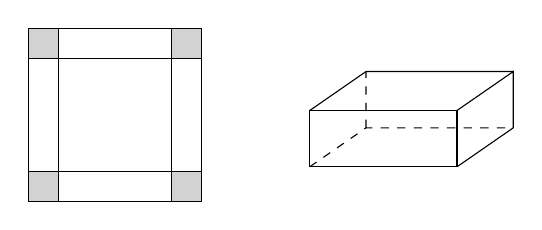
\begin{tikzpicture}[scale=.55]
  \foreach \px/\py in {0/0,3.3/0,0/3.3,3.3/3.3} \fill[gray!35] (\px,\py) rectangle ++(.7,.7);
  \draw (0,0) rectangle (4,4);
  \draw (.7,0)--(.7,4) (3.3,0)--(3.3,4) (0,.7)--(4,.7) (0,3.3)--(4,3.3);
  \begin{scope}[xshift=6.5cm,yshift=.8cm]
    \coordinate (P0) at (0,0); \coordinate (P1) at (3.4,0);
    \coordinate (Q0) at (1.3,.9); \coordinate (Q1) at (4.7,.9);
    \coordinate (T0) at (0,1.3); \coordinate (T1) at (3.4,1.3);
    \coordinate (U0) at (1.3,2.2); \coordinate (U1) at (4.7,2.2);
    \draw (P0)--(P1)--(T1)--(T0)--cycle;
    \draw (P1)--(Q1)--(U1)--(T1);
    \draw (T0)--(U0)--(U1);
    \draw[dashed] (P0)--(Q0)--(Q1) (Q0)--(U0);
  \end{scope}
\end{tikzpicture}
\end{center}
\choice{\True $\dfrac{10}3$ cm}{$10$ cm}{$20$ cm}{$\dfrac{20}3$ cm}
\loigiai{Gọi $x$ (cm), $0<x<10$, là độ dài cạnh hình vuông nhỏ cắt đi. Hộp có đáy hình vuông cạnh $20-2x$, chiều cao $x$ nên thể tích
$V(x)=x(20-2x)^2=4x^3-80x^2+400x$.
$V'(x)=12x^2-160x+400$; $V'(x)=0\Leftrightarrow x=\dfrac{10}3$ hoặc $x=10$ (loại). Lập bảng biến thiên trên $(0;10)$: $V'>0$ trên $\left(0;\dfrac{10}3\right)$, $V'<0$ trên $\left(\dfrac{10}3;10\right)$ nên $V$ lớn nhất khi $x=\dfrac{10}3$ cm.}
\end{ex}
